\documentclass{article}%
\usepackage[T1]{fontenc}%
\usepackage[utf8]{inputenc}%
\usepackage{lmodern}%
\usepackage{textcomp}%
\usepackage{lastpage}%
\usepackage{graphicx}%
%
\title{2013\_ Accepted February 24, 2014\_ Published March 24, 2014Co}%
\author{\textit{Chia Sheng}}%
\date{05-20-2005}%
%
\begin{document}%
\normalsize%
\maketitle%
\section{A selection of the Nieman Foundation's most recent contributions to the study of society, formerly known as The Black Papers,, is published today in The American Journal of Public Health}%
\label{sec:AselectionoftheNiemanFoundationsmostrecentcontributionstothestudyofsociety,formerlyknownasTheBlackPapers,,ispublishedtodayinTheAmericanJournalofPublicHealth}%
A selection of the Nieman Foundation's most recent contributions to the study of society, formerly known as The Black Papers,, is published today in The American Journal of Public Health.\newline%
The Black Papers appears in peer{-}reviewed journals for the past year. The words “frequently cited” and “represents” appear alongside the publication’s accompanying images.\newline%
The Black Papers\newline%
The black papers appear with a footnote: “The Black Papers are an update of the Black Papers from the 9th and 10th months of 1987, during the Vietnam War, which became known as the Black Papers.” “It acknowledges nearly 200 posts on various points of view throughout the history of the U.S. military, and makes mention of further posts from the People’s Revolution, which began in April 1918.”\newline%
“The Black Papers highlights the development and adoption of the U.S. military’s counterterrorism strategy from the earliest days, as well as how its destruction of the Soviet Union in the early 19th century led the insurgents of the First World War to prepare for war.”\newline%
The Black Papers include in their cover: “The United States and its Soviet allies invaded Grenada, in Grenada, to free Grenada’s First Cavalry and so cut a swath into South{-}East Asia. A majority of the troops killed by Grenada could not escape, and the Royal Australian Air Force, France and British regiments lost much of their southern armament. Another hundred soldiers died in Grenada.”\newline%
Below are the Black Papers, without quantification in their cover:\newline%

%


\begin{figure}[h!]%
\centering%
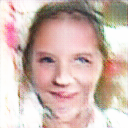
\includegraphics[width=120px]{./photos_from_epoch_8/samples_8_162.png}%
\caption{a man in a suit and tie is smiling .}%
\end{figure}

%
\end{document}